\documentclass[12pt,a4paper]{article}
 
\usepackage{float}
%für feststellen der figures und tables [H] dranschreiben
\usepackage{units}
%wird so benutzt: 
%\unit[value/Zahl]{dimension/Einheit} oder 
%\unitfrac[value/Zahl]{dimension/Einheit num/Zähler}{dimension/Einheit denum/Nenner} oder
%\nicefrac[fontcommand/Schriftart]{dimension/Einheit num/Zähler}{dimension/Einheit denum/Nenner}
\usepackage[left=2cm,right=2cm,top=2cm,bottom=2cm]{geometry}
\usepackage[utf8]{inputenc}
\usepackage[T1]{fontenc}
\usepackage{lmodern}
\usepackage[ngerman]{babel}
\usepackage{amsmath}
\usepackage{graphicx}
 
\title{Versuch AP8\\ Elektronenstrahlen}
\author{Frederik Strothmann, Henrik Jürgens}
\date{\today}
%niemals zwei überschriften direkt übereinander schreiben, also immer mindestens in einem satz was sinnvolles unter jede überschrift schreiben (bei den versuchen z.B. das versuchsziel) 
\begin{document}
%deckblatt erstellen.
\maketitle
\newpage
\tableofcontents
\newpage
\section{Einleitung}
%einleitung zu dem experiment.
%auf die einstellungen, die vor dem versuch gemacht werden, eingehen oder auf eine anleitung dazu verweisen.
Die Entdeckung der Welleneigenschaften von massebehafteten Teilchen war historisch von größter Bedeutung
für die Entwicklung der Quantenmechanik. Dabei nimmt die Schrödingergleichung als charakteristische Wellengleichung einen besonderen Stellenwert ein, da sie die Grundlage für die nicht-relativistische Quantenmechanik
bildet. In diesem Versuch führen wir zwei Teilexperimente durch, die die Teilchen- bzw. Welleneigenschaften von Elektronen demonstrieren. Mit Hilfe eines Fadenstrahlrohres bestimmen wir die spezifische Ladung e/m eines Elektrons, das im homogenen Magnetfeld eines Helmholtzspulenpaares auf eine Kreisbahn gezwungen wird.
Die Welleneigenschaften eines Elektronenstrahles wird durch Beugung von Elektronen an einer dünnen Schicht von Kohlenstoffkristallen untersucht. Mit Hilfe der bekannten Gitterkonstanten dieser Kristalle soll die Gültigkeit der DeBroglie-Beziehung nachgewiesen werden. Dabei sollen die Grenzen nicht-relativistischer Beschreibungsweise sowie der Einfluß von Wechselwirkungen zwischen den Elektronen und dem inneren Potential der Kohlenstoffkristalle berücksichtigt werden\footnote{vgl. http://www.atlas.uni-wuppertal.de/
$\sim$kind/ap22ap8neu.pdf Zielsetzung des Versuchs}.
%---------------------------------------------------------------------------------------------
%hinter der einleitung kann der allgemeine theoretische hintergrund in einer zusätzlichen section erklärt werden

\section{Verwendete Materialien}
%(immer) eine skizze oder ein foto einfügen, die geräte/materialien !nummerieren! und z.b. eine legende dazu schreiben
%falls am anfang des versuches nicht klar ist, was alles verwendet wird, wenn möglich erst am ende ein großes foto von den verwendeten materialien machen!
%-------------------------------------------------------------------------------------------
%ab hier für jeden versuchsteil einzeln, falls noch materialien hinzugenommen wurden immer im versuchsaufbau erwähnen!

Schaltskizze des Fadenstrahlrohrs zur bestimmung der spezifischen Ladung von Elektronen.

\begin{figure}[H] 
  \centering
    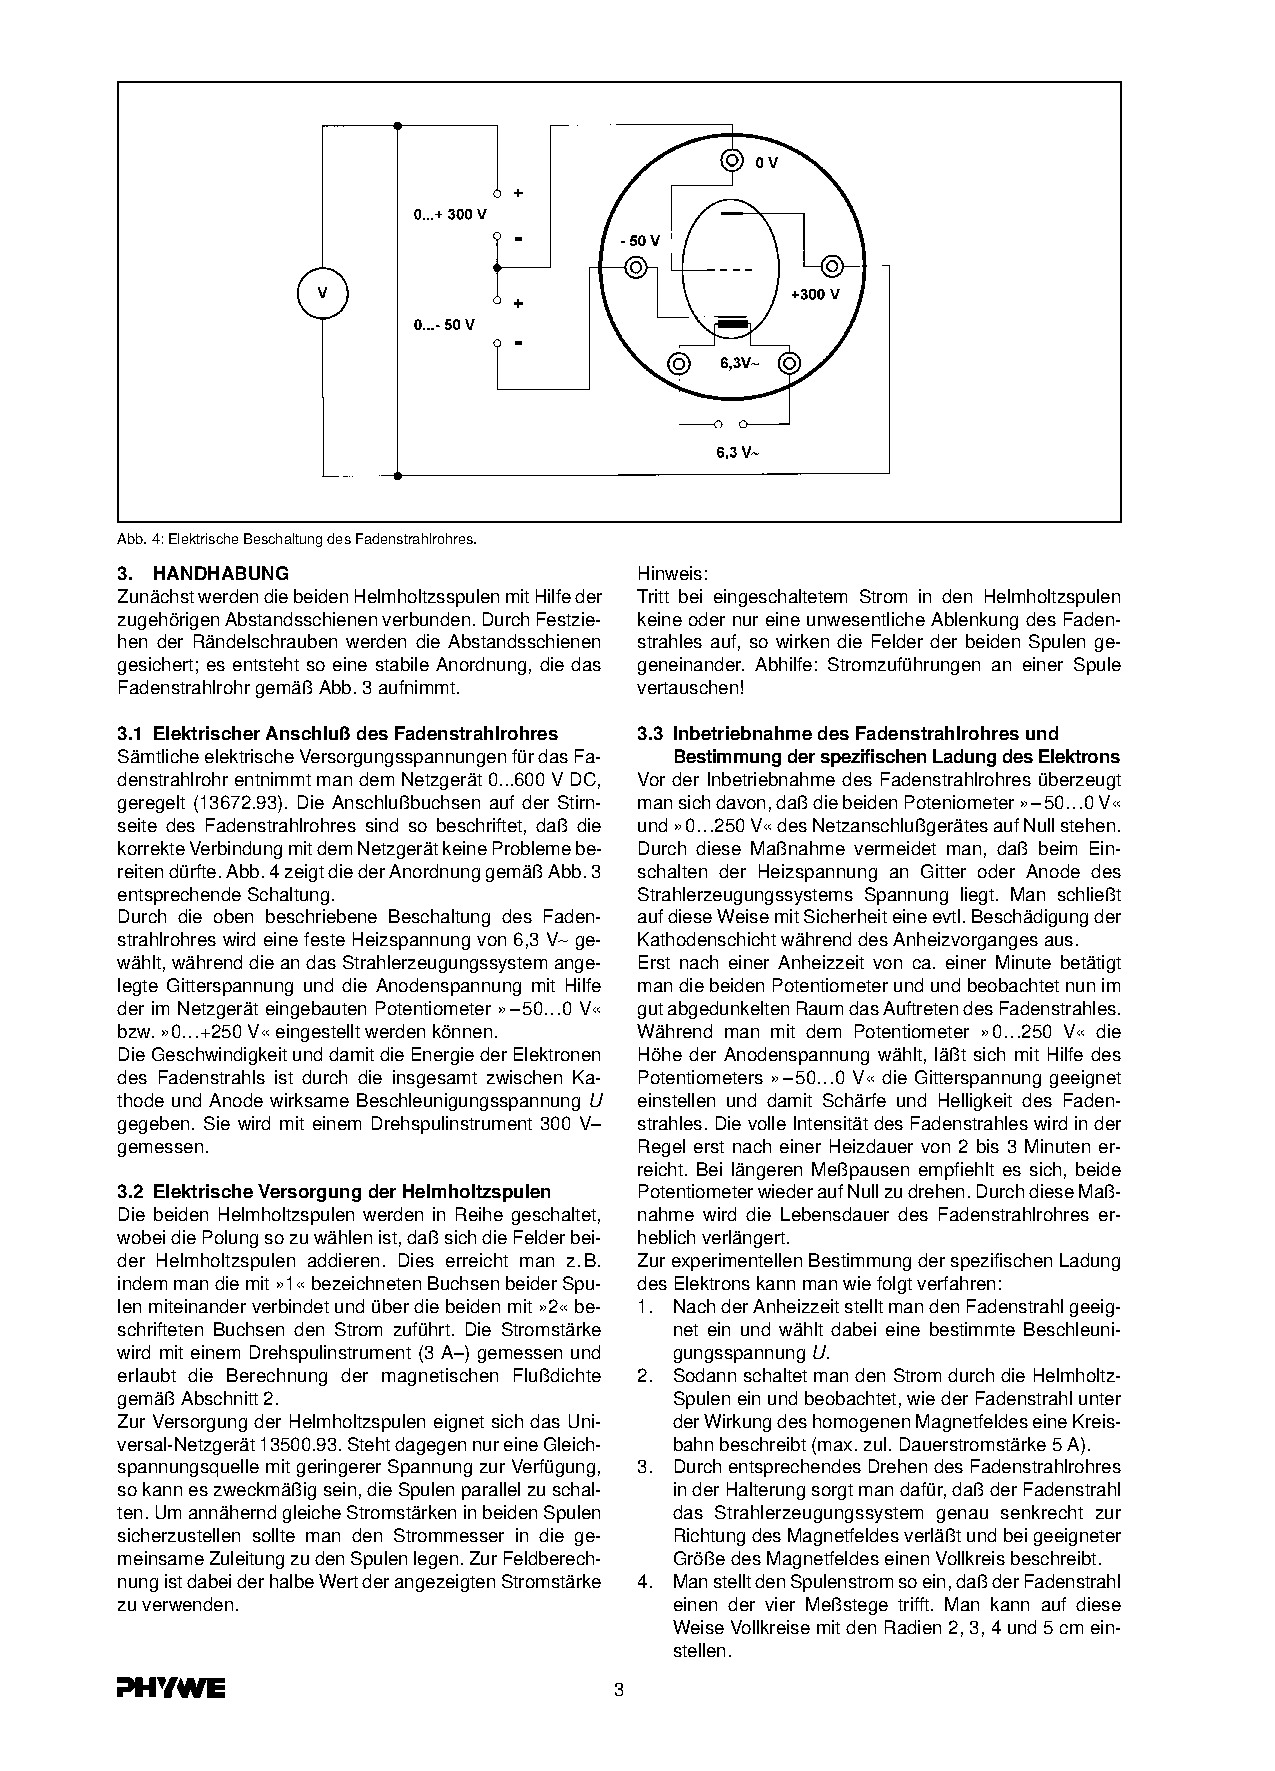
\includegraphics[trim = 10mm 210mm 10mm 10mm, clip, scale = 1]{fadenstrahlrohr.pdf}
  	\caption[Schaltskizze des Fadenstrhlrohrs]{Schaltskizze des Fadenstrhlrohrs\footnotemark}
  \label{fig:aufbau_h}
\end{figure}
\footnotetext{Abbildung entnommen von http://www.atlas.uni-wuppertal.de/$\sim$ kind/fadenstrahlrohr\_phywe\_0695900d.pdf am 24.09.2014}

\begin{itemize}
\item	6,3V:		Spannung für den Heitzdraht

\item	-50-0 V:	Spannung des Wehneltzylinder

\item	0-300V:		Beschleunigungsspannung
\end{itemize}
\newpage
Schaltskizze der Elektronenbeugungsröhre zur Bestimmung der Gitterkonstanten von Graphit.

\begin{figure}[H] 
  \centering
    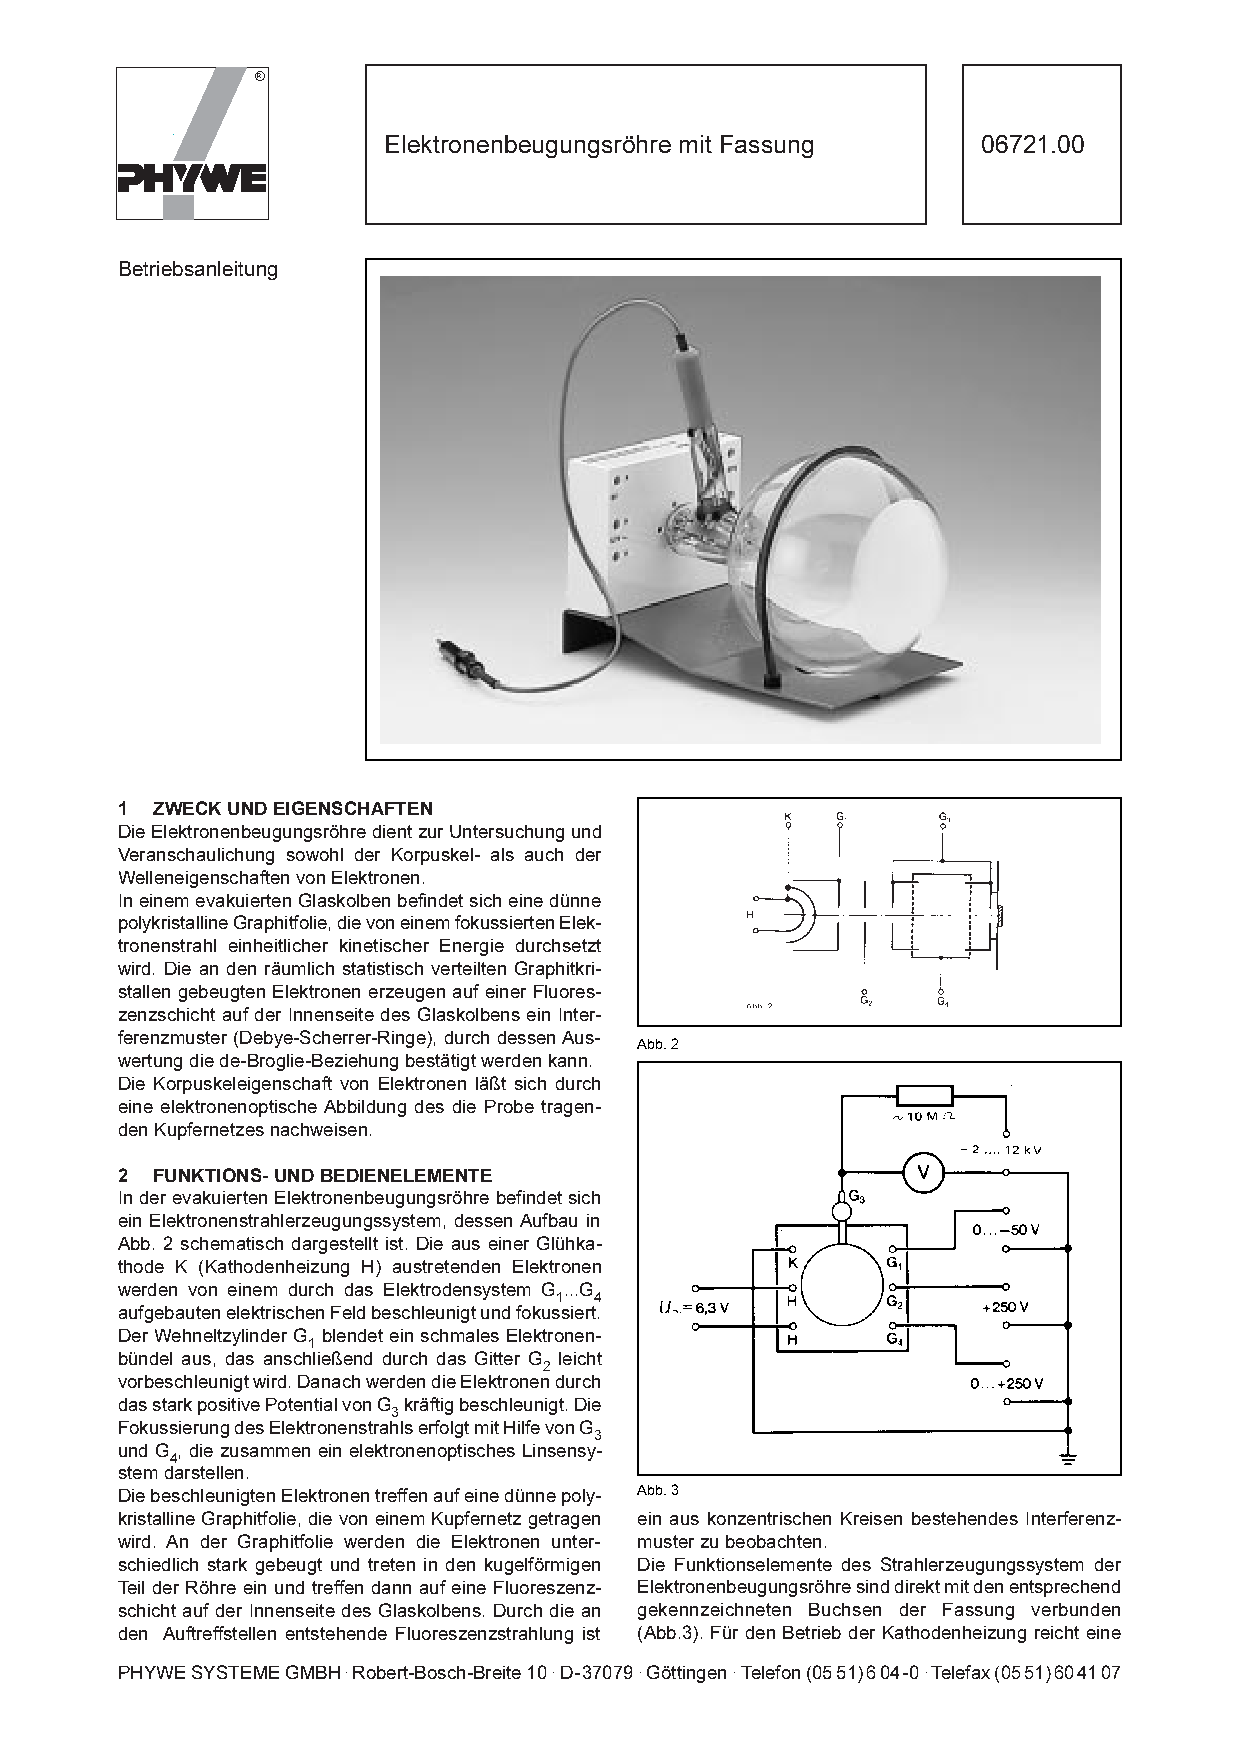
\includegraphics[trim = 105mm 47mm 10mm 178mm, clip, scale = 1]{beugungsroehre.pdf}
  	\caption[Schaltskizze der Elektronenbeugungsröhre]{Schaltskizze der Elektronenbeugungsröhre\footnotemark}
  \label{fig:aufbau_h}
\end{figure}
\footnotetext{Abbildung entnommen von http://www.atlas.uni-wuppertal.de/$\sim$   kind/beugungsroehre\_phywe\_0672100d.pdf am 24.09.2014}


\begin{itemize}
\item	H:		Kathodenheizung 

\item	K:		Glühkathode

\item	G$_1$:	Wehneltzylinder 

\item	G$_2$:	Gitter zur Vorbeschleunigung

\item	G$_3$:	Beschleunigungsgitter

\item	G$_4$:	Gitter zur Fokussierung
\end{itemize}

Das Netzgerät, dass für beide Versuchsaufbauten benötigt wird.

\begin{figure}[H] 
  \centering
    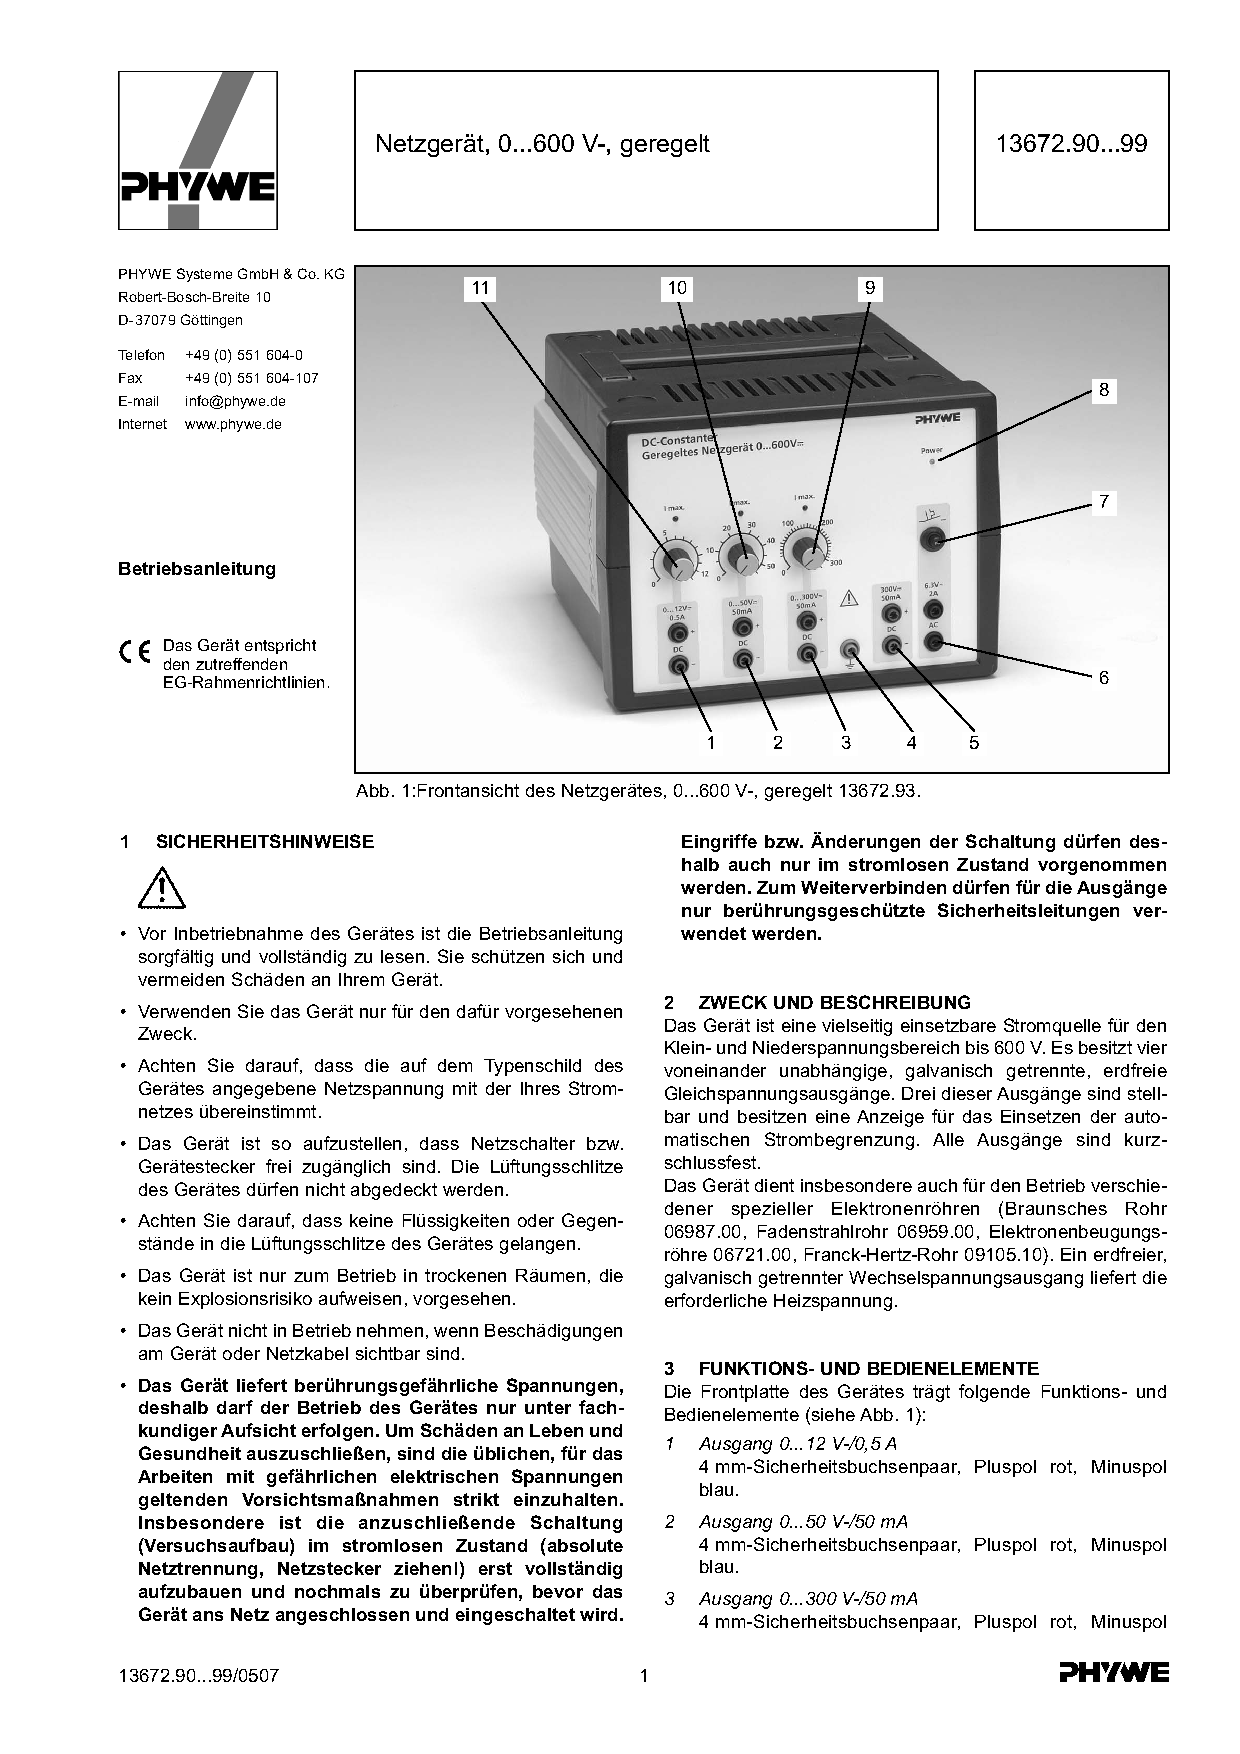
\includegraphics[trim = 60mm 165mm 10mm 40mm, clip, scale = 1]{netzteil.pdf}
  	\caption[Abbild des Netzgerätes]{Abbild des Netzgerätes\footnotemark}
  \label{fig:aufbau_h}
\end{figure}
\footnotetext{Abbildung entnommen von http://www.atlas.uni-wuppertal.de/$\sim$   kind/phywe\_600V\_netzteil\_1367293d.pdf am 24.09.2014}

\begin{enumerate}
\item	Ausgang 0-12V-/0,5A

\item	Ausgang 0-50V-/50mA

\item	Ausgang 0-300V-/50mA

\item	Anschluss 'Erde'

\item	Ausgang 300V-/50mA

\item	Ausgang 6,3V$\sim$   /2A

\item	Überstromschutzschalter für Ausgang 6,3V

\item	Einschaltkontrollleuchte

\item	Stellknopf für Ausgang 0-300V, rote Leuchtdiode zur Anzeige der Strombegrenzung

\item	Stellknopf für Ausgang 0-50V, rote Leuchtdiode zur Anzeige der Strombegrenzung

\item	Stellknopf für Ausgang 0-12V, rote Leuchtdiode zur Anzeige der Strombegrenzung
\end{enumerate}
\newpage
\section{Bestimmung der spezifischen Masse $\frac{e}{m}$}
%kurz das ziel dieses versuchsteiles ansprechen, damit keine zwei überschriften direkt übereinander stehen!
%bei schwierigeren versuchen kann auch der theoretische hintergrund erläutert werden. (mit formeln, herleitungen und erklärungen)
Ziel der Messung ist die Bestimmung der spezifischen Ladung $\frac{e}{m}$ des Elektrons mithilfe eines Fadenstrahlrohres.

\subsection{Versuchsaufbau}
%skizze zum versuchsaufbau (oder foto) einfügen,   es muss erklärt werden wie das ganze funktioniert und welche speziellen einstellungen verwendet wurden (z.b. welche knöpfe an den geräten für die messung verdreht wurden)

\begin{figure}[H] 
  \centering
    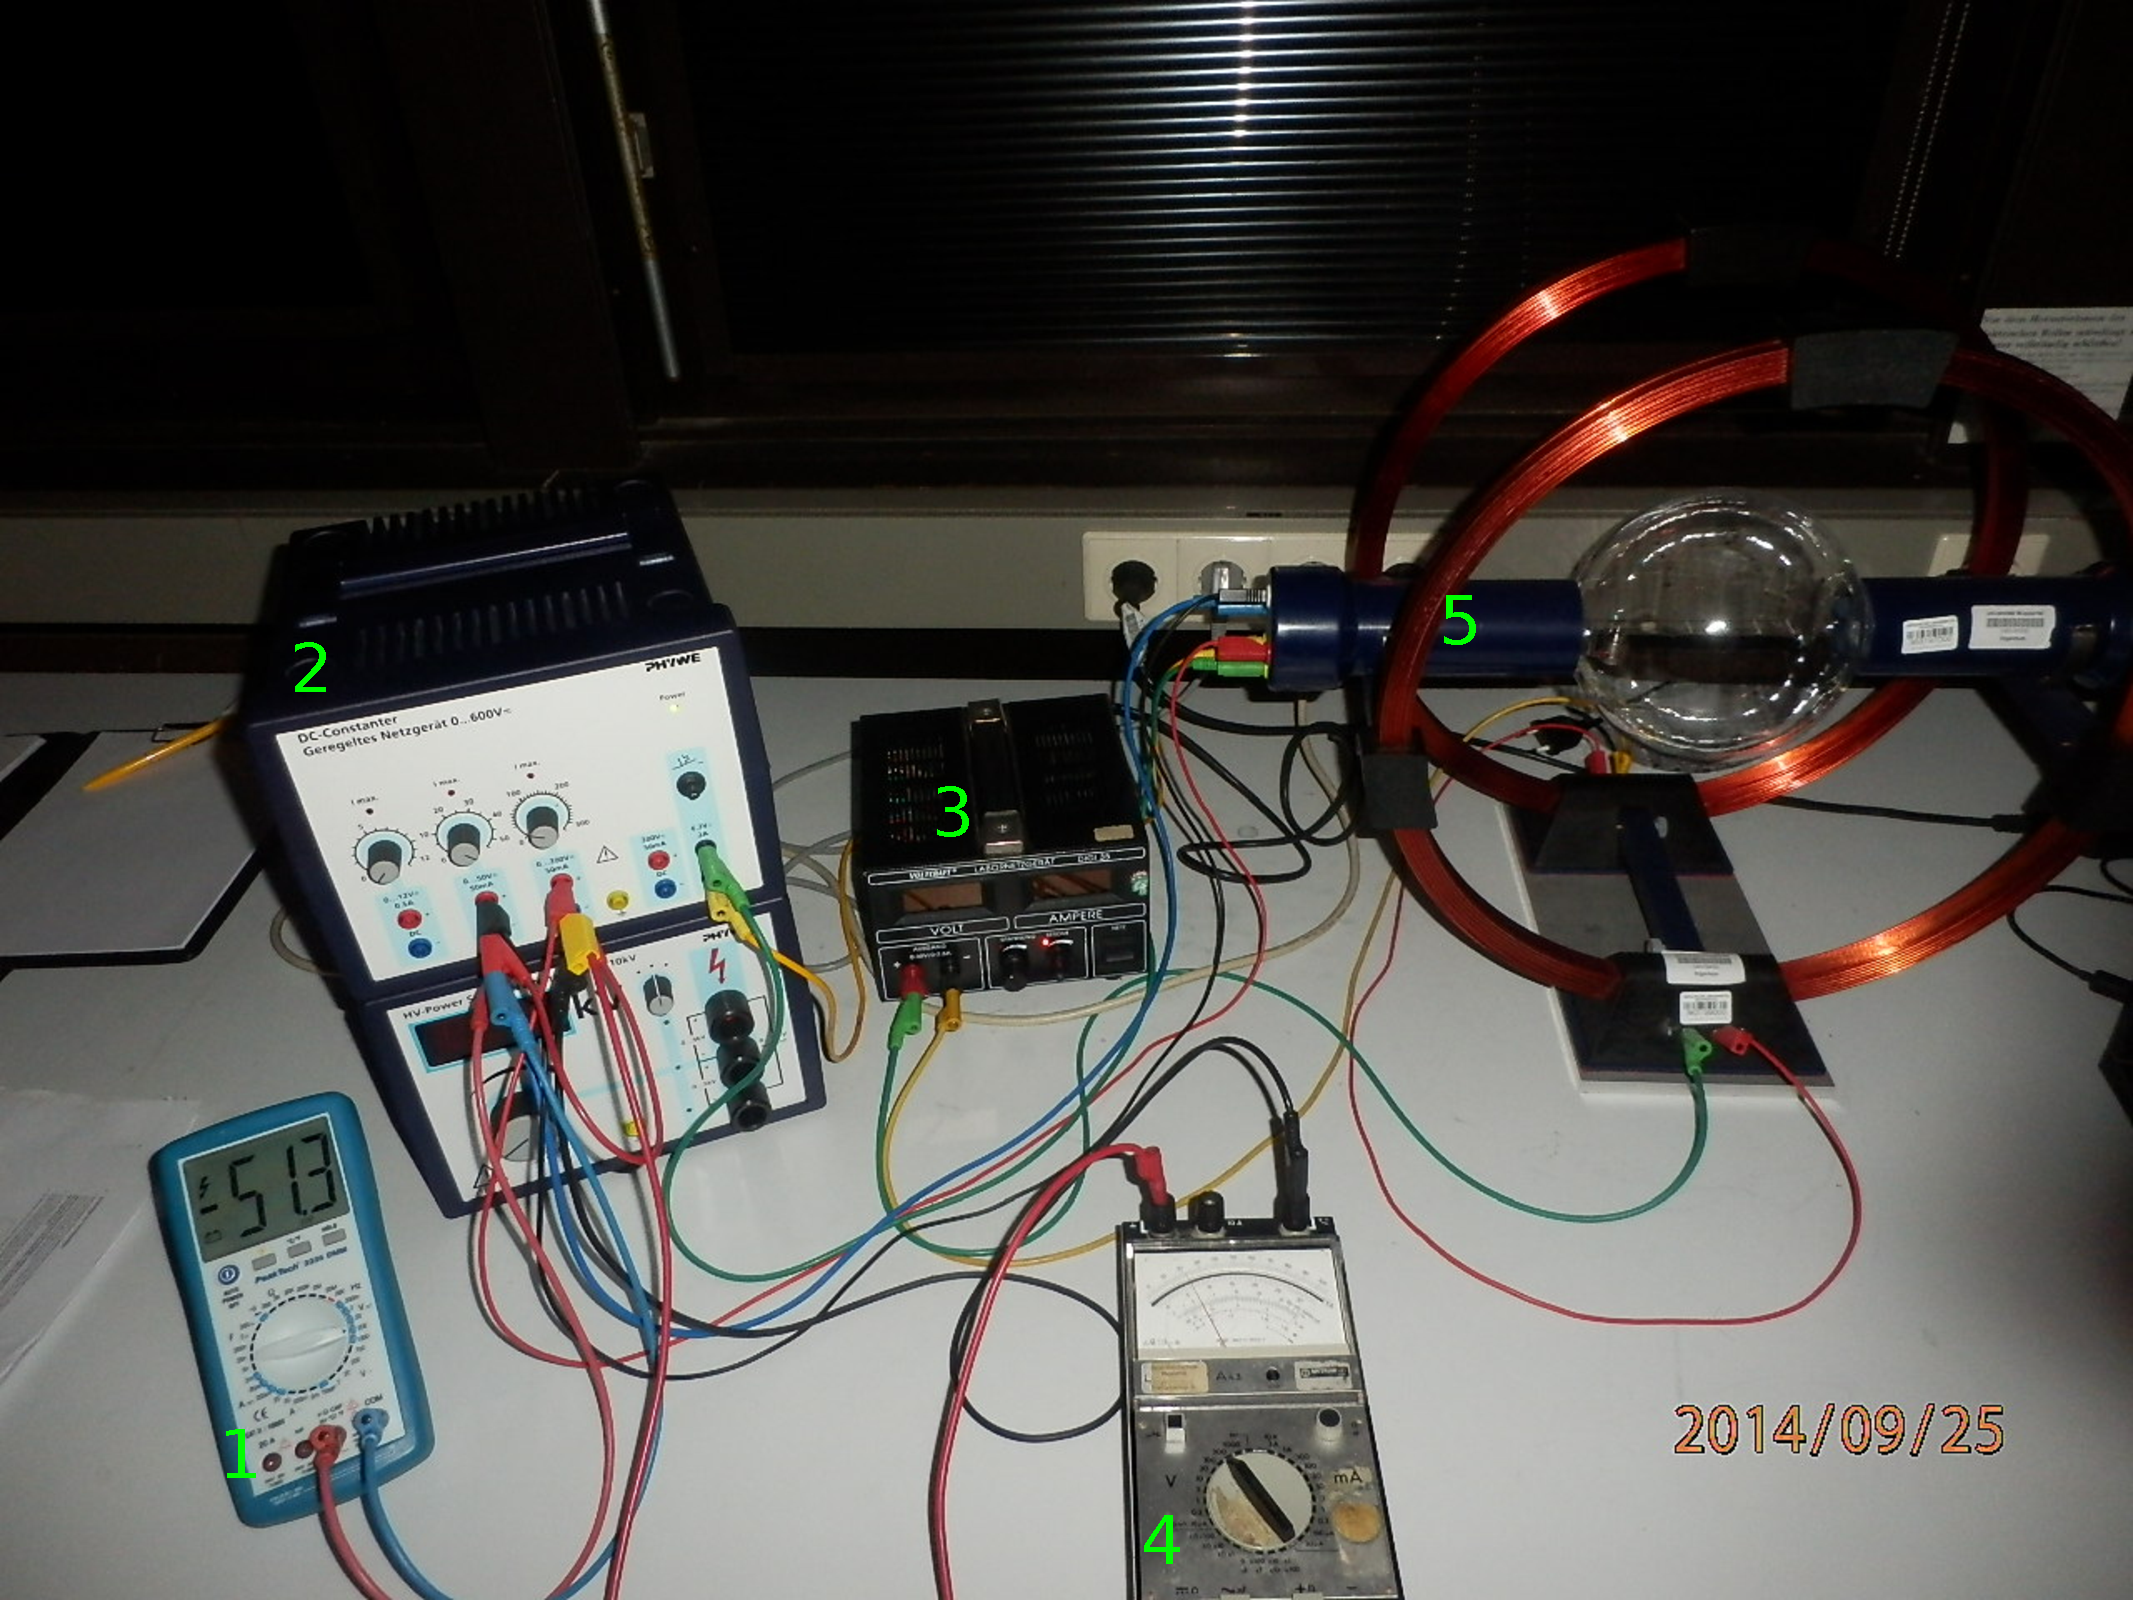
\includegraphics[scale = 0.3]{aufbau_h.pdf}
  	\caption[Abbildung des Versuchsaufbaus zur Bestimmung der spezifischen Ladung von Elektronen]{Abbildung des Versuchsaufbaus zur Bestimmung der spezifischen Ladung von Elektronen}
  \label{fig:aufbau_h}
\end{figure}

\begin{enumerate}
\item	DMM zur Messung der Gitterspannung

\item	Netzgerät zur Versorgung der Fadenstrahlrohres

\item	Netzgerät zur Versorgung der Helmholtzspule

\item	Unigor zum messen der Beschleunigungsspannung

\item	Fadenstrahlrohr und Helmholtzspule
\end{enumerate}


\subsection{Versuchsdurchführung}
%erklären, !was! wir machen, !warum! wir das machen und mit welchem ziel
%(wichtig) präzize erklären, wie bei dem versuch vorgegangen und was gemacht wurde
Zuerst werden die Helmholtzspulen in Reihe an ein Netzgerät angeschlossen, um sicherzugehen, dass durch beide Spulen der selbe Strom fließt. Es muss darauf geachtet werden, dass der Strom in beiden Spulen in die gleiche Richtung fließt, da sonst kein homogenes Magnetfeld zwischen den Spulen entsteht. Der Spulenstrom kann an der Digitalanzeige des Netzgerätes abgelesen und an einem Potentiometer verändert werden. Die Braunsche Röhre wird nach dem Schaltbild in der Versuchsanleitung\footnote{vgl. http://www.atlas.uni-wuppertal.de/
$\sim$kind/fadenstralrohr\_phywe\_0695900d.pdf Seite 3 Abb. 4} an ein weiteres Netzgerät\footnote{vgl. http://www.atlas.uni-wuppertal.de/$\sim   $kind/phywe\_600V\_netzteil\_1367293d.pdf}, welches mehrere Ausgänge hat, angeschlossen. Auf dem folgenden Bild ist der schematische Aufbau einer Braunschen Röhre abgebildet.
%bitte das Foto mit dem Schaltbild für die Braunsche Röhre einfügen
In der Mitte zwischen Wehnelt-Zylinder und Anode befindet sich das geerdete Gitter. Parallel zum Gitter und der Anode wird das Unigor (Strom- und Spannungsmessgerät) zur Messung der Beschleunigungsspannung angeschlossen, zur Überprüfung der Spannung zwischen Wehnelt-Zylinder und dem Gitter wird ein DMM parallel geschaltet. Die Spannungen zwischen Gitter und Anode, sowie zwischen Gitter und Wehnelt-Zylinder können am Netzgerät mit entsprechenden Potentiometern eingestellt werden. Die Spannung, welche am Wehnelt-Zylinder anliegt hat neben der Beschleunigung der Elektronen nach Austritt aus der Öffnung den Effekt, den Elektronenstrahl zu fokussieren. Deshalb ist es sinnvoll die Spannung am Wehnelt-Zylinder während des gesamten Versuchsteils konstant zu halten. Für verschiedene Beschleunigungsspannungen und verschiedene Spulenströme soll nun an einer im Fadenstrahlrohr vormontierten Metallleiter der Radius des Elektronenstrahls bestimmt werden (D = (4,6,8,10)cm). Aus dem Durchmesser, den angelegten Spannungen und dem Spulenstrom wird dann die spezifische Ladung $\frac{e}{m}$ errechnet.
\subsection{Verwendete Formeln}
%eine legende kann angefertigt werden, die selbstverständlichen buchstaben müssen nicht extra erklärt werden
%mit knappen erklärungen die !verwendeten! formeln, sowie die zugehörige fehlerrechnung einfügen.
\textbf{Verwendete Bezeichnungen}
\begin{enumerate}
\item $B$ := Magnetische Flussdichte im inneren der Helmholtzspulen
\item $n$ := Windungszahl
\item $I$ := Strom durch die in Reihe geschalteten Helmholtzspulen
\item $R$ := Radius der Helmholtzspulen\\
(wird aus der Versuchsanleitung ohne Fehler angenommen)
\item $\frac{e}{m}$ := Spezifische Ladung der Elektronen\\
(experimentell bestimmter Wert soll mit dem Literaturwert von $\unitfrac[1,759\cdot10^{11}]{As}{kg}$ verglichen werden)
\item $U$ := Beschleunigungsspannung
\item $r$ := Radius des Elektronenstrahles\\
(wird anhand einer in der Glaskuppel fest montierten Leiter bestimmt)
\end{enumerate}
Für die Berechung des B-Feldes verwenden wir die folgende Formel, welche sich aus dem Biot-Savart-Gesetz und der Superposition der Spulenfelder ergibt.
\begin{align}
B = \frac{8\mu_0 n I}{\sqrt{125} R}
\label{eqn:b}
\end{align}
Da $R$ als fehlerlos angenommen wurde ergibt sich nach Fehlerfortpflanzung der folgende Fehler:
\begin{align}
\Delta_B = \frac{8\mu_0 n \Delta_I}{\sqrt{125} R}
\label{eqn:b_delta}
\end{align}
Für die Berechung der spezifischen Ladung $\frac{e}{m}$ verwenden wir die Formel:
\begin{align}
\frac{e}{m} = \frac{2U}{r^2B^2}
\label{eqn:e/m}
\end{align}
Mit dem Fehler:
\begin{align}
\Delta_{\frac{e}{m}} = \sqrt{
\left(\frac{2\Delta_U}{r^2B^2}\right)^2+
\left(\frac{4U\Delta_r}{r^3B^2}\right)^2+
\left(\frac{4U\Delta_B}{r^2B^3}\right)^2}
\label{eqn:e/m_delta}
\end{align}
\subsection{Messergebnisse}
%die messwerte in !übersichtlichen! tabellen angegeben
%zu viele kleine tabellen in große tabellen überführen!
%zu große tabellen mit dem [scale]-befehl scalieren oder (falls zu lang) in zwei kleinere tabellen aufteilen
%(wichtig) vor !jeder! tabelle sagen, was gemessen wurde und wie die fehler gewählt wurden und ausreichend !erklären!, !warum! wir unsere fehler grade so gewählt haben

In der folgenden Tabelle sind die Materialeigenschaften, die zur Bestimmung des Magnetfeldes der Helmholtzspulen notwendig sind angegeben. Die Werte wurden als Fehlerlos angenommen, da sie so in der Versuchsbeschreibung angegeben sind.

\begin{table}[H]
\caption{Materialeigneschaften der Versuchsaufbaus, zur Bestimmung des Magnetfeldes der Helmholzspulen}
\begin{center}
\begin{tabular}{|l|l|l|}
\hline
Materialeigenschaften &  &  \\ \hline
$\mu_0$/($\mu$Vs/Am) & Windungsanzahl & Spulenradius/m \\ \hline
\multicolumn{1}{|r|}{1,256} & \multicolumn{1}{r|}{154} & \multicolumn{1}{r|}{0,2} \\ \hline
\end{tabular}
\end{center}
\label{tab:1_m}
\end{table}

In der folgende Tabelle befinden sich die Daten der ersten bis dritten Messung zur spezifischen Ladung von Elektronen. Der Fehler der Zylinderspannung wurde mit 1,5\% auf der Rückseite des Unigor angegeben, der Fehler für Radius wurde in der Versuchsanleitung mit >1\% angegeben, die anderen Fehler wurden alle durch die Ableseungenauigkeit bestimmt. Bei Schwankungen der Anzeige wurde zusätzlich die Hälfte des Schwankungsintervalls hinzuaddiert.

\begin{table}[H]
\caption{Messdaten der ersten bis dritten Messreihe.}
\begin{center}
\begin{tabular}{|r|r|r|r|r|r|}
\hline
\multicolumn{1}{|l|}{Strom/A} & \multicolumn{1}{l|}{Fehler/A} & \multicolumn{1}{l|}{Zylinder Spannung/V} & \multicolumn{1}{l|}{Fehler/V} & \multicolumn{1}{l|}{} & \multicolumn{1}{l|}{} \\ \hline
1,50 & 0,01 & 51,2 & 0,2 & \multicolumn{1}{l|}{} & \multicolumn{1}{l|}{} \\ \hline
\multicolumn{1}{|l|}{Spannung/V} & \multicolumn{1}{l|}{Fehler/V} & \multicolumn{1}{l|}{Beschleunigungsspannung/V} & \multicolumn{1}{l|}{Fehler/V} & \multicolumn{1}{l|}{Radius/m} & \multicolumn{1}{l|}{Fehler/m} \\ \hline
15,0 & 0,2 & 66,2 & 0,3 & 0,0200 & 0,0002 \\ \hline
36,0 & 0,5 & 87,2 & 0,6 & 0,0300 & 0,0003 \\ \hline
105 & 2 & 156 & 2 & 0,0400 & 0,0004 \\ \hline
189 & 3 & 240 & 3 & 0,0500 & 0,0005 \\ \hline \hline
\multicolumn{1}{|l|}{Strom/A} & \multicolumn{1}{l|}{Fehler/A} & \multicolumn{1}{l|}{Zylinder Spannung/V} & \multicolumn{1}{l|}{Fehler/V} & \multicolumn{1}{l|}{} & \multicolumn{1}{l|}{} \\ \hline
1,70 & 0,01 & 51,2 & 0,2 & \multicolumn{1}{l|}{} & \multicolumn{1}{l|}{} \\ \hline
\multicolumn{1}{|l|}{Spannung/V} & \multicolumn{1}{l|}{Fehler/V} & \multicolumn{1}{l|}{Beschleunigungsspannung/V} & \multicolumn{1}{l|}{Fehler/V} & \multicolumn{1}{l|}{Radius/m} & \multicolumn{1}{l|}{Fehler/m} \\ \hline
30,0 & 0,5 & 81 & 0,5 & 0,0200 & 0,0002 \\ \hline
65 & 1 & 116 & 1 & 0,0300 & 0,0003 \\ \hline
145 & 2 & 196 & 2 & 0,0400 & 0,0004 \\ \hline
259 & 4 & 310 & 4 & 0,0500 & 0,0005 \\ \hline \hline
\multicolumn{1}{|l|}{Strom/A} & \multicolumn{1}{l|}{Fehler/A} & \multicolumn{1}{l|}{Zylinder Spannung/V} & \multicolumn{1}{l|}{Fehler/V} & \multicolumn{1}{l|}{} & \multicolumn{1}{l|}{} \\ \hline
2,00 & 0,01 & 51,2 & 0,2 & \multicolumn{1}{l|}{} & \multicolumn{1}{l|}{} \\ \hline
\multicolumn{1}{|l|}{Spannung/V} & \multicolumn{1}{l|}{Fehler/V} & \multicolumn{1}{l|}{Beschleunigungsspannung/V} & \multicolumn{1}{l|}{Fehler/V} & \multicolumn{1}{l|}{Radius/m} & \multicolumn{1}{l|}{Fehler/m} \\ \hline
45,0 & 0,7 & 96,2 & 0,7 & 0,0200 & 0,0002 \\ \hline
100 & 2 & 151 & 2 & 0,0300 & 0,0003 \\ \hline
220 & 3 & 271 & 3 & 0,0400 & 0,0004 \\ \hline
\end{tabular}
\end{center}
\label{tab:1_1}
\end{table}
\newpage

\subsection{Auswertung}
%zuerst !alle! errechneten werte entweder in ganzen sätzen aufzählen, oder in tabellen (übersichtlicher) dargestellen, sowie auf die verwendeten formeln verweisen (die referenzierung der formel kann in der überschrift stehen)
%kurz erwähnen (vor der tabelle), warum wir das ganze ausrechnen bzw. was wir dort ausrechnen
%danach histogramme und plots erstellen, wobei wenn möglich funktionen durch die plots gelegt werden (zur not können auch splines benutzt werden, was aber angegeben werden muss)
%bei fits immer die funktion und das reduzierte chiquadrat mit angegeben, wobei auf verständlichkeit beim entziffern der zehnerpotenzen geachtet werden muss z.b. f(x)=(wert+-fehler)\cdot10^{irgendeine zahl}\cdot x + (wert+-fehler)\cdot10^{irgendeine zahl}
%bei jedem fit erklären, nach welchem zusammenhang gefittet wurde und warum!
%bei plots darauf achten, dass die achsenbeschriftung (auch die tics) die richtige größe haben und die legende im plot nicht die messwerte verdeckt
%kurz die aufgabenstellung abgehandeln

Aus den Gemessenen Daten (Tabelle \ref{tab:1_1}) soll die spezifische Ladung von Elektronen bestimmt werde. Dafür wurde zu erste das Magnetfeld der Helmholzspulen aus dem Strom und den Materialeigenschaften (Tabelle \ref{tab:1_m}) nach Gleichung \ref{eqn:b} und der Fehler nach Gleichung \ref{eqn:b_delta}  bestimmt. Es ergaben sich die folgenden Werte.

\begin{table}[H]
\caption{Magnetfelder der drei Messungen}
\begin{center}
\begin{tabular}{|r|r|r|}
\hline
\multicolumn{1}{|l|}{Messung} & \multicolumn{1}{l|}{Magnetfeld/T$\cdot 10^{-6}$} & \multicolumn{1}{l|}{Fehler/T$\cdot 10^{-6}$} \\ \hline
1 & 1176 & 7 \\ \hline
2 & 1038 & 7 \\ \hline
3 & 1384 & 7 \\ \hline
\end{tabular}
\end{center}
\label{tab:aus_b}
\end{table}

Mit Gleichung \ref{eqn:e/m} wurden dann die spezifische Ladung von Elektronen bestimmt, der Fehler wurde mit Gleichung \ref{eqn:e/m_delta} berechnet.

\begin{table}[H]
\caption{Spezifische Ladung von Elektronen für verschiedene Radien und Beschleunigungsspannungen}
\begin{center}
\begin{tabular}{|r|r|}
\hline
\multicolumn{1}{|l|}{Messung 1.} & \multicolumn{1}{l|}{} \\ \hline
\multicolumn{1}{|l|}{e/m/($10^{11}$As/kg)} & \multicolumn{1}{l|}{Fehler/($10^{11}$As/kg)} \\ \hline
2,93 & 0,07 \\ \hline
1,87 & 0,05 \\ \hline
1,77 & 0,05 \\ \hline
1,79 & 0,05 \\ \hline \hline
\multicolumn{1}{|l|}{Messung 2.} & \multicolumn{1}{l|}{} \\ \hline
\multicolumn{1}{|l|}{e/m/($10^{11}$As/kg)} & \multicolumn{1}{l|}{Fehler/($10^{11}$As/kg)} \\ \hline
3,07 & 0,08 \\ \hline
1,80 & 0,04 \\ \hline
1,81 & 0,05 \\ \hline
1,78 & 0,05 \\ \hline \hline
\multicolumn{1}{|l|}{Messung 3.} & \multicolumn{1}{l|}{} \\ \hline
\multicolumn{1}{|l|}{e/m/($10^{11}$As/kg)} & \multicolumn{1}{l|}{Fehler/($10^{11}$As/kg)} \\ \hline
2,51 & 0,06 \\ \hline
1,75 & 0,04 \\ \hline
1,77 & 0,05 \\ \hline
\end{tabular}
\end{center}
\label{tab:aus_e/m}
\end{table}

Gemittelt ergibt sich ein Wert von \unit[(1,79 $\pm$0,01)$\cdot 10^{11}$]{$\frac{\text{As}}{\text{kg}}$}, dabei wurde der erste Wert jeder Messung nicht mit einbezogen, da die Spannung am Wehneltzylinder für zu kleine Radien der Beschleunigungsspannung entgegen wirkte und somit das Ergebnis unserer Messung stark verfälscht wurde.
\newpage
\subsection{Diskussion}
%(immer) die gemessenen werte und die bestimmten werte über die messfehler mit literaturwerten oder untereinander vergleichen
%in welchem fehlerintervall des messwertes liegt der literaturwert oder der vergleichswert?
%wie ist der relative anteil des fehlers am messwert und damit die qualität unserer messung?
%in einem satz erklären, wie gut unser fehler und damit unsere messung ist
%kurz erläutern, wie systematische fehler unsere messung beeinflusst haben könnten
%(wichtig) zum schluss ansprechen, in wie weit die ergebnisse mit der theoretischen vorhersage übereinstimmen
%--------------------------------------------------------------------------------------------
%falls tabellen mit den messwerten zu lang werden, kann die section mit den messwerten auch hinter der diskussion angefügt bzw. eine section mit dem anhang eingefügt werden.

Es wurde eine spezifische Ladung von \unit[1,76 $\cdot 10^{11}$]{$\frac{As}{kg}$} für Elektronen erwartet, der von uns bestimmte Wert liegt bei \unit[(1,79 $\pm$0,03)$\cdot 10^{11}$]{$\frac{\text{As}}{\text{kg}}$}. Der Anteil der des Fehlers am Messwert liegt bei 1,83\%. Die prozentuale Abweichung vom Literaturwert beträgt 1,77\%, was ein guter Wert ist, da der Literaturwert im ersten Fehlerintervall des bestimmten Wertes liegt. Eine Relativistische Betrachtung ist in diesem Versuchsteil nicht nötig, da sich die Elektronen mit maximal 3,5\% der Lichtgeschwindigkeit bewegen.

\section{Beugung von Elektronenstrahlen, Verifikation der DeBroglie-Beziehung}
%kurz das ziel dieses versuchsteiles ansprechen, damit keine zwei überschriften direkt übereinander stehen!
%bei schwierigeren versuchen kann auch der theoretische hintergrund erläutert werden. (mit formeln, herleitungen und erklärungen)
Ziel des Versuchs ist die Bestimmung der Gitterkonstanten $d_1$ und $d_2$ einer Graphitschicht anhand des Interferenzmusters, welches durch den Beschuss mit Elektronen entsteht. Dabei sollen relativistische Effekte berücksichtigt werden.
\subsection{Versuchsaufbau}
%skizze zum versuchsaufbau (oder foto) einfügen,   es muss erklärt werden wie das ganze funktioniert und welche speziellen einstellungen verwendet wurden (z.b. welche knöpfe an den geräten für die messung verdreht wurden)

Versuchsaufbau zur Bestimmung der Gitterkonstanten von Graphit.

\begin{figure}[H] 
  \centering
    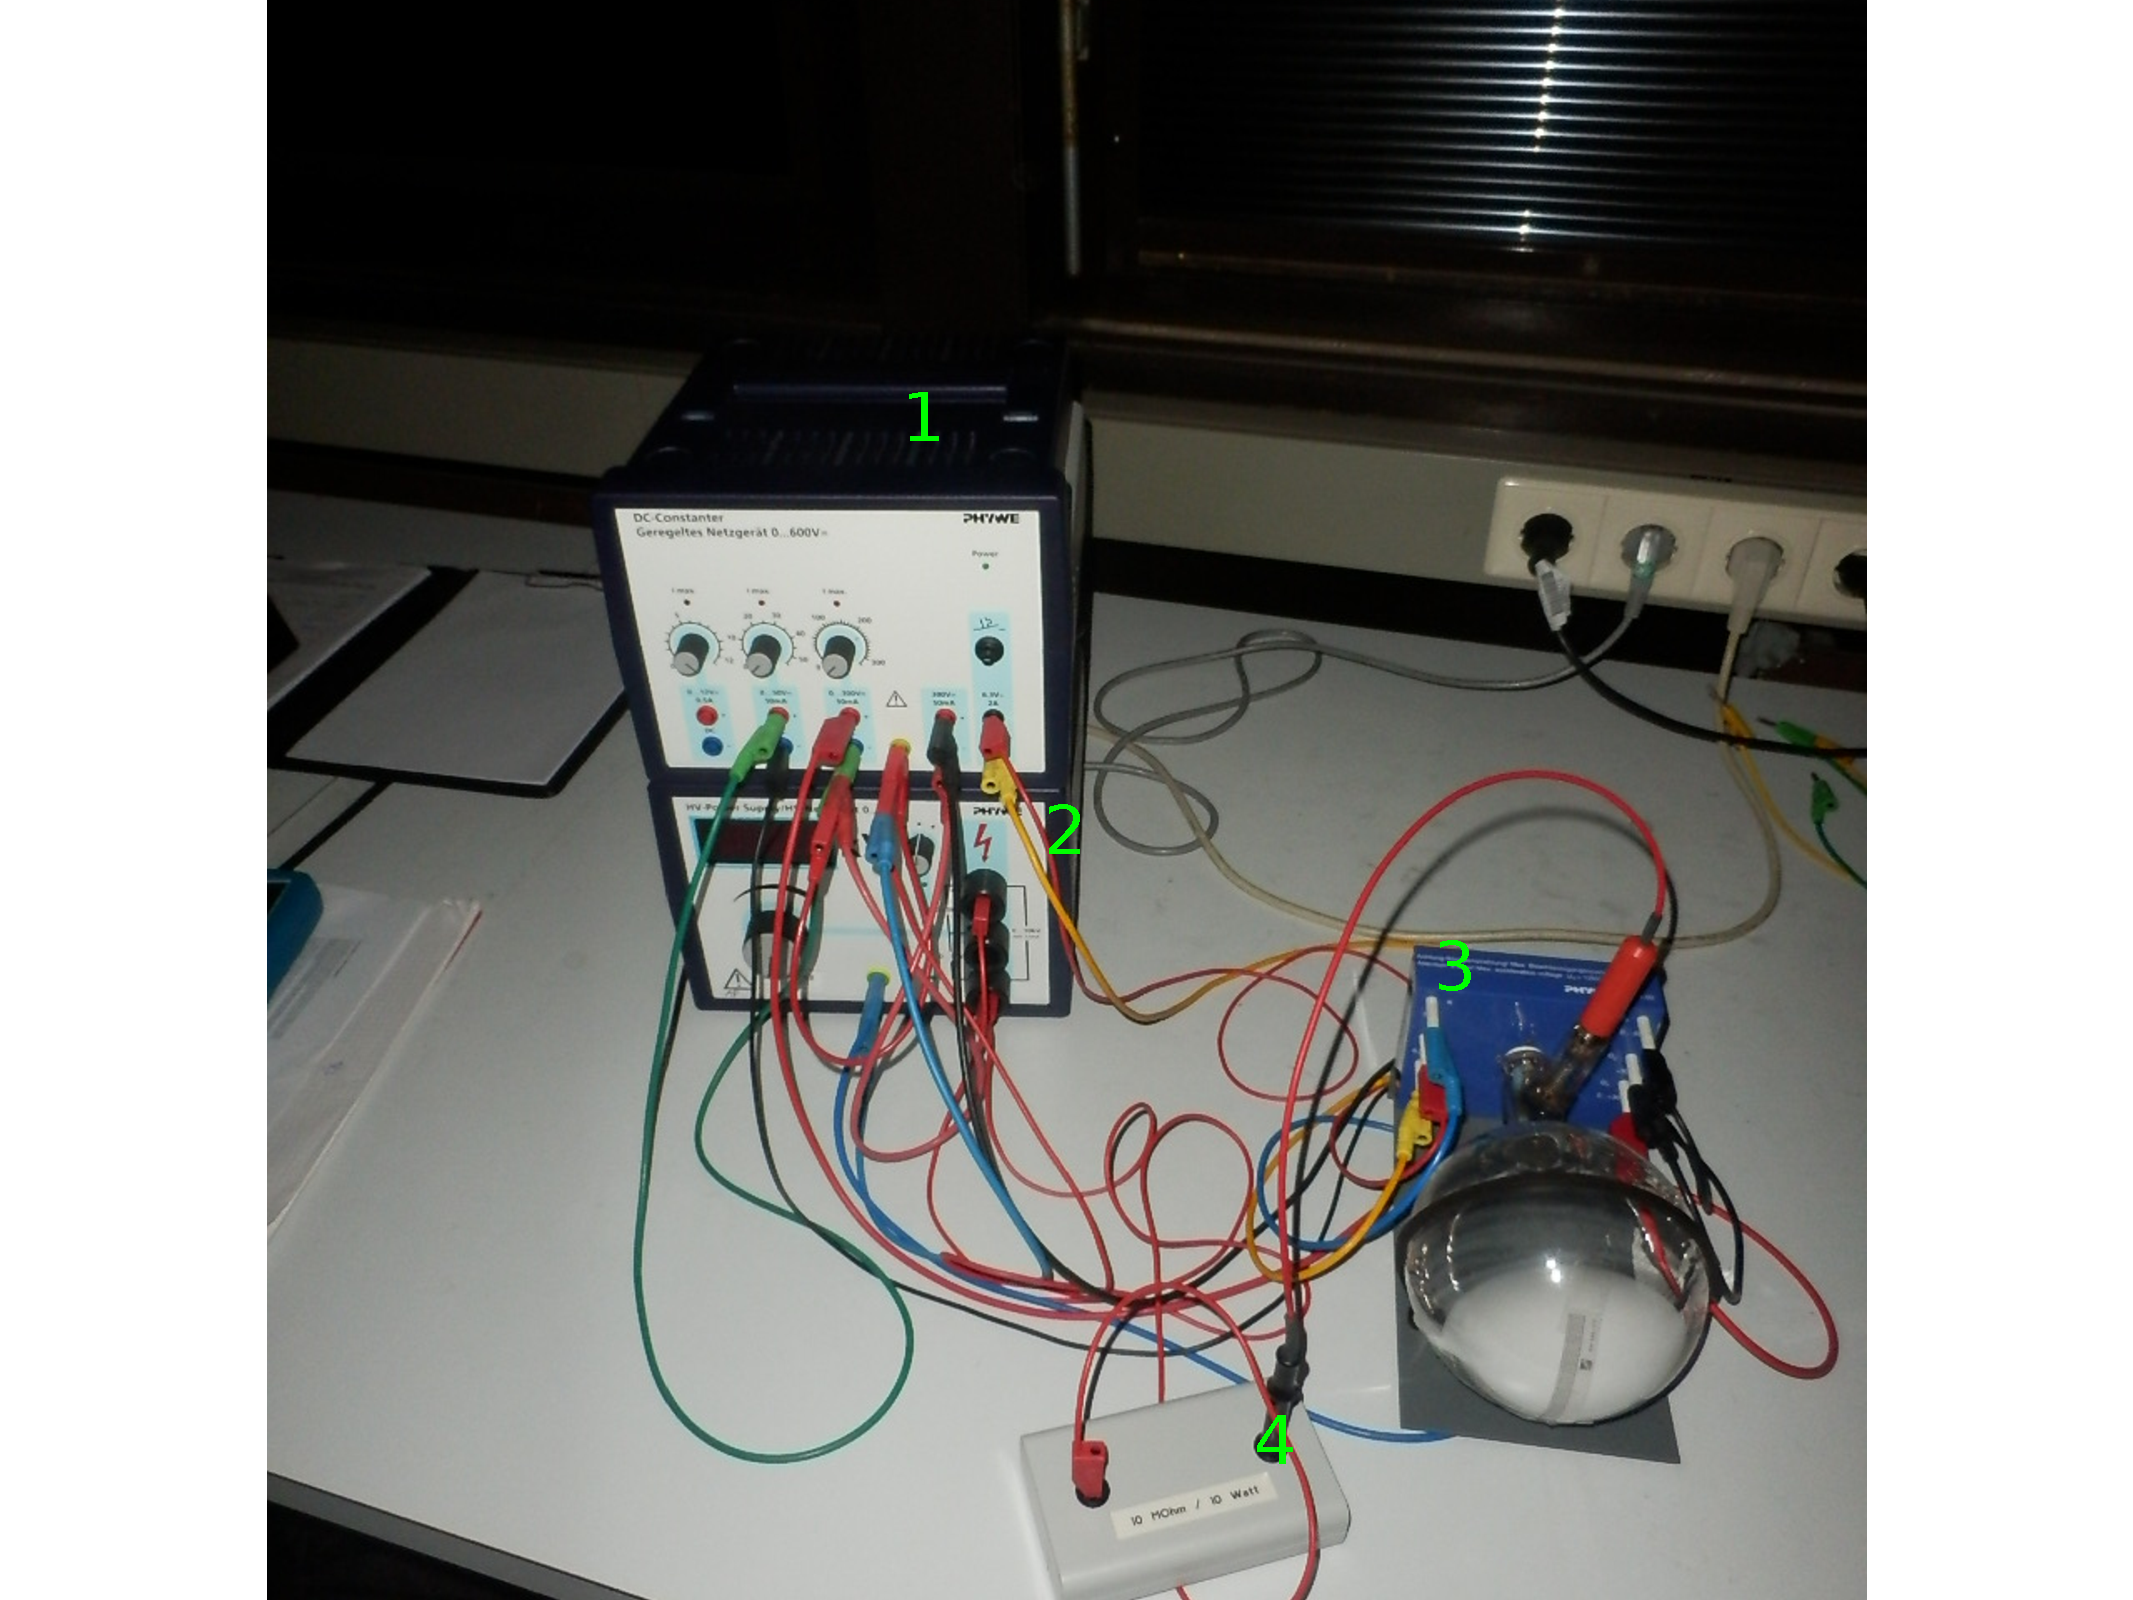
\includegraphics[scale = 0.3]{aufbau_b.pdf}
  	\caption[Abbildung des Versuchsaufbaus zur Bestimmung der spezifischen Ladung von Elektronen]{Abbildung des Versuchsaufbaus zur Bestimmung der spezifischen Ladung von Elektronen}
  \label{fig:aufbau_h}
\end{figure}

\begin{enumerate}
\item	Netzgerät

\item	Hochspannungsnetzgerät

\item	Elektronenbeugungsröhre mit Fassung

\item	10m$\Omega$ Vorwiederstand, damit der Anodenstrom den Wert von 1mA nicht überschreitet
\end{enumerate}


\subsection{Versuchsdurchführung}
%erklären, !was! wir machen, !warum! wir das machen und mit welchem ziel
%(wichtig) präzize erklären, wie bei dem versuch vorgegangen und was gemacht wurde
Zuerst schalten wir die Elektronenbeugungsröhre gemäß des Schaltbildes in der Versuchsbeschreibung\footnote{vgl. http://www.atlas.uni-wuppertal.de/
$\sim$kind/beugungsroehre\_phywe\_0672100d.pdf Seite 1 Abb. 2 und 3}. Die Spannung am Wehnelt-Zylinder ist für die Fokussierung des Elektronenstrahls verantwortlich, weshalb wir diese maximal gewählt haben, die Beschleunigungsspannung der Braunschen Röhre ist dagegen eher unwichtig und wir haben sie deshalb minimal gewählt. Da die Energiezunahme der Elektronen durch die Spannung am Wehnelt-Zylinder im Vergleich zur Energiezunahme durch die dahinter geschaltetete Anodenspannung von 2 bis 12kV zu vernachlässigen ist, wird diese im folgenden nicht weiter berücksichtigt. Die Elektronen erreichen bei einer Spannung von 12kV eine Geschwindigkeit von etwas weniger als 22\% der Lichtgeschwindigkeit. Deshalb ist in diesem Versuchsteil eine relativistische Betrachtung bzw. eine Abschätzung des Fehlers durch relativistische Effekte sinnvoll. Nachdem die Kathode aufgeheizt und die Spannungen angeschaltet sind, kann am Schirm der Elektronenbeugungsröhre das Interferenzmuster, welches sich aus der Bragg-Gleichung ergibt, beobachtet und mit der hinter dem Schirm angeklebten Millimeterfolie vermessen werden\footnote{Herleitung der Bragg-Gleichung/Bedingung für konstruktive Interferenz http://de.wikipedia.org/wiki/Bragg-Gleichung}.
Da die Kristallgitter statistisch angeordnet sind und wir in diesem Versuch nur die ersten Maxima für beide bekannten Gitterkonstanten $d_1$ und $d_2$ untersuchen, können wir über den Durchmesser der am Schirm leuchtenden Kreise, die durch die Interferenz der Elektronen am Kristallgitter entstehen, die Gitterkonstanten experimentell verifizieren und damit die DeBroglie-Beziehung nachweisen.
\subsection{Verwendete Formeln}

%eine legende kann angefertigt werden, die selbstverständlichen buchstaben müssen nicht extra erklärt werden
%mit knappen erklärungen die !verwendeten! formeln, sowie die zugehörige fehlerrechnung einfügen.
\textbf{Verwendete Bezeichnungen}
\begin{enumerate}
\item $d_{1,2}$ := Gitterkonstanten von Graphit\\
(als Literaturwerte wurden in der Anleitung 213 und 123 pm a angegeben)
\item $\theta_{1,2}$ := Braggwinkel
\item $lambda$ := DeBroglie-Wellenlänge
\item $U$ := Beschleunigungsspannung
\item $m_e$ := Elektronenmasse\\
(neben dieser Naturkonstanten tauchen die selbsterklärenden Konstanten $h$:= Planck. WQ, $e$ := Elementarladung und $c$ := Lichtgeschwindigkeit auf)
\item $D_{1,2}$ := Durchmesser des durch das jeweils erste Maximum erzeugten Interferenzkreises (je nach Gitterkonstante)
\item $D$ := Durchmessder des Glaskolbens
\item $m_{1,2}$ := Steigung, welche aus dem Plot mit Hilfe von Gnuplot bestimmt wird.
\item $\gamma$ := Lorentzfaktor
\item $U'$ := korrigierte Spannung\\
(wird anstatt einer relativen Massenänderung eingeführt, sodass weiterhin die Ruhemasse der Elektronen sowie Gleichung \ref{eqn:Geradenbeziehung} verwendet werden kann)
\end{enumerate}
Für die Herleitung der Verwendeten Steigungsformel der Geraden, aus der $d_1$ und $d_2$ bestimmt wird, schreiben wir die Bragg-Bedingung und die Formel für die Berechung des Braggwinkels $\theta$, welche sich aus der Zeichnung in der Versuchsbeschreibung\footnote{vgl. http://www.atlas.uni-wuppertal.de/
$\sim$kind/beugungsroehre\_phywe\_0672100d.pdf Seite 2 Abb. 5} ergibt kurz auf.\\
Bragg-Bedingung für das erste Maximum abhängig von $d_1$ und $\theta_1$ bzw. $d_2$ und $\theta_2$:
\begin{align}
2d_{1,2}\sin(\theta_{1,2}) = \lambda =
\sqrt{\frac{h^2}{2m_eeU}}
\end{align}
Bragg Winkel:
\begin{align}
\theta_{1,2} = \frac{1}{4}\arcsin(D_{1,2}/D)
\end{align}
Daraus ergibt sich für kleine Winkel d.h. $\sin(\theta) \sim   eq \theta$ und nach einsetzen von $\theta$ in die Bragg-Bedingung die Lineare Beziehung
\begin{align}
D_{1,2} = \frac{D\sqrt{\frac{2h^2}{m_ee}}}{d_{1,2}}\frac{1}{\sqrt{U}}
\label{eqn:Geradenbeziehung}
\end{align}\\
zwischen $D_{1,2}$ und $\frac{1}{\sqrt{U}}$.\\
Wir berechnen aus den Steigungen dieser Geraden dann die beiden Gitterkonstanten nach der folgenden Formel:
\begin{align}
d_{1,2} = \frac{D\sqrt{\frac{2h^2}{m_ee}}}{m_{1,2}}
\label{eqn:d}
\end{align}
Mit dem Fehler:
\begin{align}
\Delta_{d_{1,2}} = \frac{D\sqrt{\frac{2h^2}{m_ee}}}{m_{1,2}^2}\Delta_{m_{1,2}}
\label{eqn:d_delta}
\end{align}
Der Durchmesser des Glaskolbens, sowie die Naturkonstanten wurden dabei als Fehlerlos angenommen.\\
\textbf{Zum Schluss wollen wir unsere Rechnung noch einmal mit Hilfe der speziellen Relativitätstheorie korrigieren.}\\
Dazu schauen wir uns nochmal Formel \ref{eqn:Geradenbeziehung} an und überlegen uns welche Größen wir transformieren müssen. Da die aus dem Loborsystem bewegten Teilchen die Elektronen sind, welche mit fast 22\% der Lichtgeschwindigkeit an uns vorbeirasen, müssen wir die relativistische Massenzunahme der Elektronen berücksichtigen.
Die Elektronenmasse $m_e'$ berechnet sich dabei nach der folgenden Formel ($m_e$ bleibt im folgenden immer die Ruhemasse der Elektronen):
\begin{align}
m_e' = \gamma m_e = \frac{m_e}{\sqrt{1-\frac{v^2}{c^2}}}
\end{align}
$v$ müssen wir dabei genaugenommen ebenfalls relativistisch ausrechnen:
\begin{align}
v = \sqrt{\frac{2eU}{m_e'}} = \sqrt{\frac{2eU\sqrt{1-\frac{v^2}{c^2}}}{m_e}}
\end{align}
Wir potenzieren mit 4 und erhalten eine quadratische Gleichung für $v^2$:
\begin{align}
v^4 + v^2\frac{4 e^2 U^2}{m_e^2 c^2} - \frac{4 e^2 U^2}{m_e^2} = 0
\end{align}
Diese lösen wir nach $v^2$ auf und sehen sofort, dass nur die positive Lösung für $v^2$ infrage kommt, da $v^2$ in den reellen Zahlen immer positiv ist:
\begin{align}
v^2_{1,2} = -\frac{2e^2U^2}{m_e^2c^2} \pm \sqrt{\frac{4e^4U^4}{m_e^4c^4}+\frac{4e^2U^2}{me^2}} = \frac{2eU}{m_e}\left(\pm\sqrt{\frac{e^2U^2}{m_e^2c^4}+1}-\frac{eU}{m_e c^2}\right)
\end{align}
Da wie bereits erwähnt nur '+' sinnvoll ist können wir nun $v^2$ in unsere korrigierte Masse einsetzen und danach diese wiederum in Formel \ref{eqn:Geradenbeziehung} einsetzen.
Es ergibt sich exakt die gleiche lineare Beziehung zwischen $\left(\frac{1}{U^2}-\frac{v^2}{U^2c^2}\right)^{\frac{1}{4}}$ und $D_{1,2}$ wie zwischen $D_{1,2}$ und $\frac{1}{\sqrt{U}}$ nach Formel \ref{eqn:Geradenbeziehung}.
Daher ist es sinnvoll Formel \ref{eqn:Geradenbeziehung} für die relativistische Rechnung mit dem korrigierten U':
\begin{align}
U' = \frac{1}{\sqrt{\frac{1}{U^2}-\frac{v^2}{U^2c^2}}}
\label{eqn:u_r}
\end{align}
weiterzuverwenden. Also:
\begin{align}
D_{1,2} = \frac{D\sqrt{\frac{2h^2}{m_ee}}}{d_{1,2}}\frac{1}{\sqrt{U'}}
\label{eqn:d_r}
\end{align}
Und analog die Gitterkonstante aus der Steigung des korrigierten Plots nach Gleichung \ref{eqn:d} zu bestimmen.
Für U' werden dabei weiterhin die Ablesefehler von U verwendet, da eine weitere Fehlerfortpflanzung den Fehler von U' nur minimal verändern und dies nichts an der Steigung der mit Gnuplot gefitteten Geraden ändern würde. Der Fehler der aus dem Plot errechneten Steigung $m_{1,2}$ würde sich ebenfalls nur unwesentlich vergrößern.
\subsection{Messergebnisse}
%die messwerte in !übersichtlichen! tabellen angegeben
%zu viele kleine tabellen in große tabellen überführen!
%zu große tabellen mit dem [scale]-befehl scalieren oder (falls zu lang) in zwei kleinere tabellen aufteilen
%(wichtig) vor !jeder! tabelle sagen, was gemessen wurde und wie die fehler gewählt wurden und ausreichend !erklären!, !warum! wir unsere fehler grade so gewählt haben

In der folgenden Tabelle sind die Materialeigenschaften und Einstellungen des Netzgerätes zur Bestimmung der Gitterkonstanten von Graphit eingetragen.

\begin{table}[H]
\caption{Materialeigenschaften und Einstellungen}
\begin{center}
\begin{tabular}{|l|}
\hline
Materialeigenschaften und Einstellungen \\ \hline
Glaskolbendurchmesser/m \\ \hline
\multicolumn{1}{|r|}{0,127} \\ \hline
Wehneltzylinderspannung/V \\ \hline
\multicolumn{1}{|r|}{-50} \\ \hline
Vorbeschleunigungsspannung/V \\ \hline
\multicolumn{1}{|r|}{0} \\ \hline
\end{tabular}
\end{center}
\label{tab:a_2_m}
\end{table}

\newpage
In der folgenden Tabelle sind die Messdaten zur Bestimmung der zwei Gitterkonstanten von Graphit. Die Fehler wurden durch die Ableseungenauigkeit bestimmt. Für die Beschleunigungsspannung ergab sich ein Fehler von 0,1kV und für den Durchmesser ein Fehler von 0,001m.

\begin{table}[H]
\caption{Messung der Durchmesser in Abhängigkeit der Beschleunigungsspannung}
\begin{center}
\begin{tabular}{|r|r|r|}
\hline
$U_\text{A}$/kV & Durchmesser\_1/m & Durchmesser\_2/m \\ \hline
4,5 & 0,022 & 0,04 \\ \hline
5,5 & 0,020 & 0,035 \\ \hline
6,5 & 0,019 & 0,033 \\ \hline
7,5 & 0,017 & 0,031 \\ \hline
8,5 & 0,016 & 0,03 \\ \hline
9,5 & 0,015 & 0,029 \\ \hline
10,5 & 0,015 & 0,027 \\ \hline
11,5 & 0,014 & 0,025 \\ \hline
\end{tabular}
\end{center}
\label{tab:a_2}
\end{table}

\begin{table}[H]
\caption{Daten für den Plot des ersten Kreises im nicht relativistischen Fall}
\begin{center}
\begin{tabular}{|r|r|r|r|}
\hline
\multicolumn{1}{|l|}{$1/\sqrt{U_A}$/(1/$\sqrt{V}$)} & \multicolumn{1}{l|}{Durchmesser/m} & \multicolumn{1}{l|}{Fehler(1/$\sqrt{V}$)} & \multicolumn{1}{l|}{Fehler/m} \\ \hline
0,0149 & 0,022 & 0,0002 & 0,001 \\ \hline
0,0135 & 0,020 & 0,0001 & 0,001 \\ \hline
0,01240 & 0,019 & 0,00009 & 0,001 \\ \hline
0,01155 & 0,017 & 0,00008 & 0,001 \\ \hline
0,01085 & 0,016 & 0,00006 & 0,001 \\ \hline
0,01026 & 0,015 & 0,00005 & 0,001 \\ \hline
0,00976 & 0,015 & 0,00005 & 0,001 \\ \hline
0,00933 & 0,014 & 0,00004 & 0,001 \\ \hline
\end{tabular}
\end{center}
\label{tab:p_1}
\end{table}

\begin{table}[H]
\caption{Daten für den Plot des zweiten Kreises im nicht relativistischem Fall}
\begin{center}
\begin{tabular}{|r|r|r|r|}
\hline
\multicolumn{1}{|l|}{$1/\sqrt{U_A}$/(1/$\sqrt{V}$)} & \multicolumn{1}{l|}{Durchmesser/m} & \multicolumn{1}{l|}{Fehler(1/$\sqrt{V}$)} & \multicolumn{1}{l|}{Fehler/m} \\ \hline
0,0149 & 0,04 & 0,0002 & 0,001 \\ \hline
0,0135 & 0,035 & 0,0001 & 0,001 \\ \hline
0,01240 & 0,033 & 0,00009 & 0,001 \\ \hline
0,01155 & 0,031 & 0,00008 & 0,001 \\ \hline
0,01085 & 0,03 & 0,00006 & 0,001 \\ \hline
0,01026 & 0,029 & 0,00005 & 0,001 \\ \hline
0,00976 & 0,027 & 0,00005 & 0,001 \\ \hline
0,00933 & 0,025 & 0,00004 & 0,001 \\ \hline
\end{tabular}
\end{center}
\label{tab:p_2}
\end{table}


\begin{table}[H]
\caption{Daten für den Plot des ersten Kreises im relativistischen Fall}
\begin{center}
\begin{tabular}{|r|r|r|r|}
\hline
\multicolumn{1}{|l|}{$1/\sqrt{U_A'}$/(1/$\sqrt{V}$)} & \multicolumn{1}{l|}{Durchmesser/m} & \multicolumn{1}{l|}{Fehler/(1/$\sqrt{V}$)} & \multicolumn{1}{l|}{Fehler/m} \\ \hline
0,0148 & 0,022 & 0,0002 & 0,001 \\ \hline
0,0134 & 0,020 & 0,0001 & 0,001 \\ \hline
0,01228 & 0,019 & 0,00009 & 0,001 \\ \hline
0,01142 & 0,017 & 0,00008 & 0,001 \\ \hline
0,01071 & 0,016 & 0,00007 & 0,001 \\ \hline
0,01012 & 0,015 & 0,00005 & 0,001 \\ \hline
0,00961 & 0,015 & 0,00005 & 0,001 \\ \hline
0,00917 & 0,014 & 0,00004 & 0,001 \\ \hline
\end{tabular}
\end{center}
\label{tab:p_1_r}
\end{table}

\begin{table}[H]
\caption{Daten für den Plot des zweiten Kreises im relativistischen Fall}
\begin{center}
\begin{tabular}{|r|r|r|r|}
\hline
\multicolumn{1}{|l|}{$1/\sqrt{U_A'}$/(1/$\sqrt{V}$)} & \multicolumn{1}{l|}{Durchmesser/m} & \multicolumn{1}{l|}{Fehler(1/$\sqrt{V}$)} & \multicolumn{1}{l|}{Fehler/m} \\ \hline
0,0148 & 0,04 & 0,0002 & 0,001 \\ \hline
0,0134 & 0,035 & 0,0001 & 0,001 \\ \hline
0,01228 & 0,033 & 0,00009 & 0,001 \\ \hline
0,01142 & 0,031 & 0,00008 & 0,001 \\ \hline
0,01071 & 0,03 & 0,00006 & 0,001 \\ \hline
0,01012 & 0,029 & 0,00005 & 0,001 \\ \hline
0,00961 & 0,027 & 0,00005 & 0,001 \\ \hline
0,00917 & 0,025 & 0,00005 & 0,001 \\ \hline
\end{tabular}
\end{center}
\label{tab:p_2_r}
\end{table}
\newpage
\subsection{Auswertung}
%zuerst !alle! errechneten werte entweder in ganzen sätzen aufzählen, oder in tabellen (übersichtlicher) dargestellen, sowie auf die verwendeten formeln verweisen (die referenzierung der formel kann in der überschrift stehen)
%kurz erwähnen (vor der tabelle), warum wir das ganze ausrechnen bzw. was wir dort ausrechnen
%danach histogramme und plots erstellen, wobei wenn möglich funktionen durch die plots gelegt werden (zur not können auch splines benutzt werden, was aber angegeben werden muss)
%bei fits immer die funktion und das reduzierte chiquadrat mit angegeben, wobei auf verständlichkeit beim entziffern der zehnerpotenzen geachtet werden muss z.b. f(x)=(wert+-fehler)\cdot10^{irgendeine zahl}\cdot x + (wert+-fehler)\cdot10^{irgendeine zahl}
%bei jedem fit erklären, nach welchem zusammenhang gefittet wurde und warum!
%bei plots darauf achten, dass die achsenbeschriftung (auch die tics) die richtige größe haben und die legende im plot nicht die messwerte verdeckt
%kurz die aufgabenstellung abgehandeln

Es sollen die zwei Gitterkonstanten von Graphit bestimmt werden. Dazu wurde der Durchmesser $D_{1,2}$ des bei konstruktiver Interferenz entstehenden Kreises in Abhängigkeit von $\frac{1}{\sqrt{\text{U}_{\text{A}}}}$ aufgetragen. Da ein linearer Zusammenhang erwartet wird, werden die Messdaten mit f(x)=m$\cdot$x+b gefittet.
Für den ersten Kreis ergibt sich der folgende Plot (Daten aus Tabelle \ref{tab:p_1_r}).

\begin{figure}[H] 
  \centering
    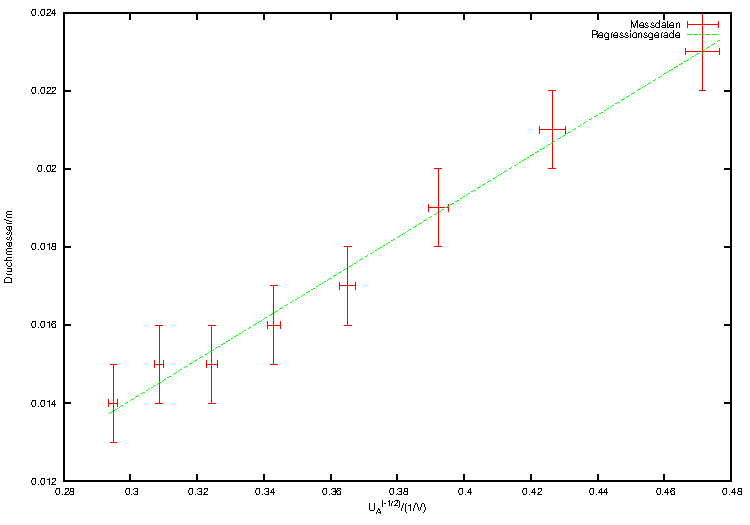
\includegraphics[scale = 1]{kreis_1.pdf}
  	\caption[Graphische Darstellung der Messdaten, des ersten Ringes, mit linearem Fit]{Graphische Darstellung der Messdaten, des ersten Ringes, mit linearem Fit}
  \label{fig:plot_1}
\end{figure}

Die gefittete Funktion ergab sich mit f(x)=(1,45$\pm$0,06)$\cdot$x-(0,0005$\pm$0,0008), das reduzierte $\chi^2$ ergibt sich mit 0,11.
\newpage
Für den zweiten Kreis ergibt sich der folgende Plot (Daten aus Tabelle \ref{tab:p_2_r}).
\begin{figure}[H] 
  \centering
    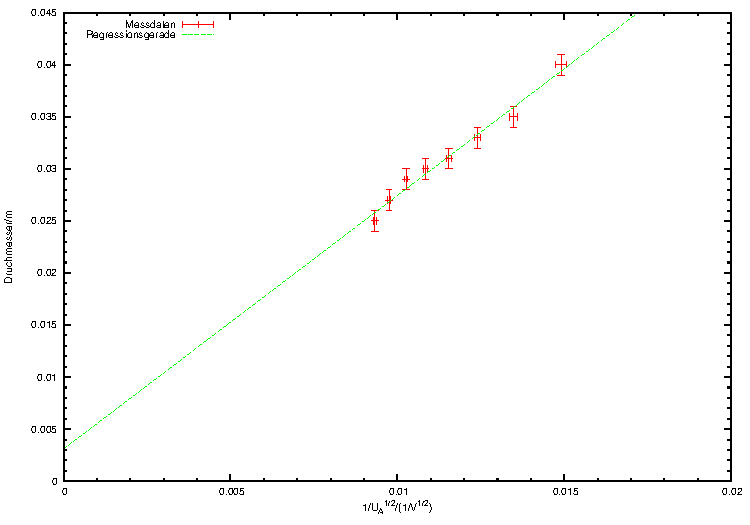
\includegraphics[scale = 1]{kreis_2.pdf}
  	\caption[Graphische Darstellung der Messdaten, des zweiten Kreises, mit linearem Fit]{Graphische Darstellung der Messdaten, des zweiten Kreises, mit linearem Fit}
  \label{fig:plot_1}
\end{figure}

Der Fit ergab sich mit f(x)=(2,4$\pm$0,1)$\cdot$x+(0,003$\pm$0,002), das reduzierte $\chi^2$ ergibt sich dabei mit 0,52.

Aus der Steigung sollen die Gitterkonstanten berechnet werden, dazu wird Gleichung \ref{eqn:d} und Gleichung \ref{eqn:d_delta} für den Fehler verwendet. Für die erste Steigung ergibt sich eine Gitterkonstante von \unit[(215$\pm$8)]{pm} und für die zweite Steigung ergibt sich eine Gitterkonstante von \unit[(127$\pm$7)]{pm}.

\newpage
Unter relativistischer Betrachtung ergeben sich die folgenden Plots (Daten aus Tabelle \ref{tab:p_1}) .
\begin{figure}[H] 
  \centering
    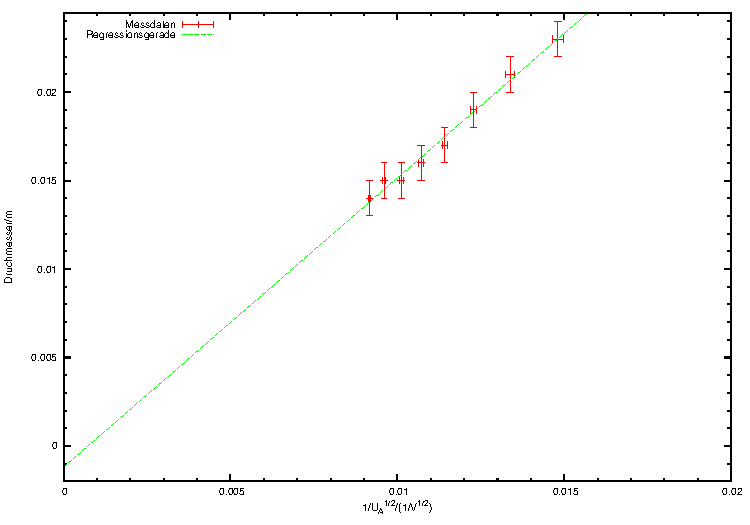
\includegraphics[scale = 1]{kreis_1_r.pdf}
  	\caption[Graphische Darstellung der Messdaten, des ersten Ringes, mit linearem Fit, unter relativistischer Betrachtung]{Graphische Darstellung der Messdaten, des ersten Ringes, mit linearem Fit, unter relativistischer Betrachtung}
  \label{fig:plot_1}
\end{figure}

Die gefittete Funktion ergab sich mit f(x)=(1,44$\pm$0,06)$\cdot$x-(0,0008$\pm$0,0007), das reduzierte $\chi^2$ ergibt sich mit 0,11.
\newpage
Für den zweiten Kreis ergibt sich der folgende Plot (Daten aus Tabelle \ref{tab:p_2}).

\begin{figure}[H] 
  \centering
    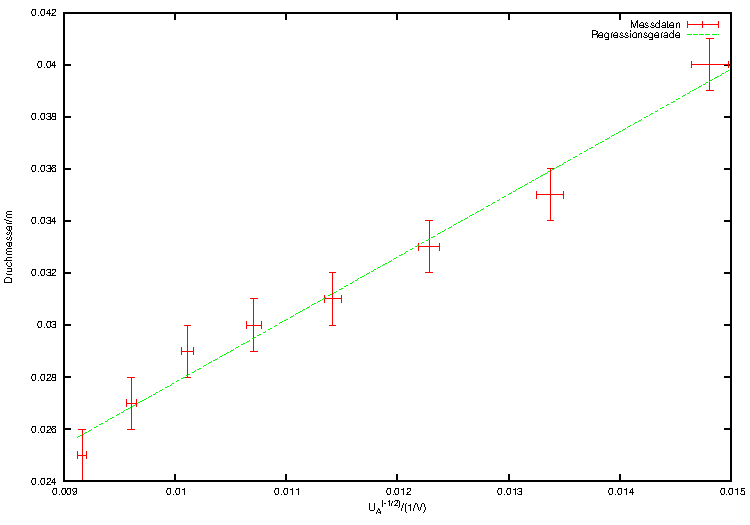
\includegraphics[scale = 1]{kreis_2_r.pdf}
  	\caption[Graphische Darstellung der Messdaten, des zweiten Kreises, mit linearem Fit, unter relativistischer Betrachtung]{Graphische Darstellung der Messdaten, des zweiten Kreises, mit linearem Fit, unter relativistischer Betrachtung}
  \label{fig:plot_1}
\end{figure}

Der Fit ergab sich mit f(x)=(2,4$\pm$0,1)$\cdot$x+(0,003$\pm$0,002), das reduzierte $\chi^2$ ergibt sich dabei mit 0,52.

Aus den relativistischen Werte wurden die Gitterkonstanten nach Gleichung \ref{eqn:d_r} bestimmt. Für die erste Steigung ergibt sich eine Gitterkonstante von \unit[(216$\pm$9)]{pm} und für die zweite Steigung ergibt sich eine Gitterkonstante von \unit[(129$\pm$7)]{pm}.
\newpage
\subsection{Diskussion}
%(immer) die gemessenen werte und die bestimmten werte über die messfehler mit literaturwerten oder untereinander vergleichen
%in welchem fehlerintervall des messwertes liegt der literaturwert oder der vergleichswert?
%wie ist der relative anteil des fehlers am messwert und damit die qualität unserer messung?
%in einem satz erklären, wie gut unser fehler und damit unsere messung ist
%kurz erläutern, wie systematische fehler unsere messung beeinflusst haben könnten
%(wichtig) zum schluss ansprechen, in wie weit die ergebnisse mit der theoretischen vorhersage übereinstimmen
%--------------------------------------------------------------------------------------------
%falls tabellen mit den messwerten zu lang werden, kann die section mit den messwerten auch hinter der diskussion angefügt bzw. eine section mit dem anhang eingefügt werden.

Nach der Versuchsbeschreibung wurden Gitterkonstanten von \unit[123]{pm} und \unit{213}[pm] erwartet. Die nicht relativistisch bestimmten Gitterkonstanten ergeben sich mit \unit{(127$\pm$7)}[pm] und \unit[(215$\pm$8)]{pm}. Der prozentuale Anteil des Fehlers am ersten Messwert liegt bei 5,5\%, beim zweiten Messwert bei 3,7\%. Der erste Messwert weicht um 0,7\% und der zweite Messwert um 3,5\% vom jeweiligen Literaturwert ab. Die Literaturwerte liegen beide im ersten Fehlerintervall der gemessenen Werte.
Bei der relativistischen Betrachtung ergaben sich Gitterkonstanten von \unit[(129$\pm$8)]{pm} und \unit[(216$\pm$9)]{pm}. Der prozentuale Anteil des Fehlers am ersten Messwert beträgt 5,4\% und beim zweitem Messwert 4,2\%. Die prozentuale Abweichung der Messwerte zum Literaturwert beträgt 4,6\% für die erste Gitterkonstante und 1,8\% für die zweite Gitterkonstante. Die Literaturwerte liegen wieder im ersten Fehlerintervall der bestimmten Gitterkonstanten,
jedoch hat sich die Abweichung der Messwerte zum Literaturwert bei der relativistischen Betrachtung vergrößert, was nicht zu erwarten war. Die relativistisch bestimmten Gitterkonstanten haben sich im Vergleich zu den nicht relativistisch berechneten Konstanten um den Faktor 1,011  (für beide Werte gleich) vergrößert. Wenn man $\sin(\frac{1}{4}\arcsin(x)))$ um die Stelle x=0 entwickelt, erhält man: $\sin(\frac{1}{4}\arcsin(x)))=\frac{1}{4}(x+\frac{5}{32} \text{x}^3 + \mathcal{O}(\text{x}^5) $). An dieser Tailorreihe kann man gut erkennen, wenn man z.B. probehalber die ersten beiden Werte ($x+\frac{5}{32} \text{x}^3\simeq\frac{D_{1,2}}{D}$) als bessere Näherung in Formel \ref{eqn:Geradenbeziehung} einsetzt, dass durch die zuerst verwendete Näherung von $\frac{x}{4}=\sin(\frac{1}{4}\arcsin(x))$ ein Wert bestimmt wird, der für den größeren am Schirm bestimmten Durchmesser ca. 1\% zu groß ist, und für den kleineren bestimmten Durchmesser ca. 0,5\% zu groß ist. Damit heben sich die beiden systematischen Fehler zum Großteil auf, sodass sich die Verschlechterung der Messwerte nach der relativistischen Betrachtung erklärt. Eine relativistische Betrachtung wäre also auch in diesem Versuchsteil nicht notwendig gewesen, da die Messfehler im Vergleich zum Einfluss des Korrekturfaktors einen viel größeren Anteil an den Messwerten haben.



\section{Fazit}
%im fazit nochmal alles zusammenfassen und den verlauf der messung abschätzen
%gravierende sytematische probleme bei den messungen nochmal betonen und die wertigkeit unserer ergebnisse einordnen
Zusammenfassend sind die Messungen gut verlaufen und bei allen bestimmten Werten liegen die Literaturwerte im ersten Fehlerintervall der bestimmten Werte. Bei der Bestimmung der spezifischen Ladung wurden die Messwerte des \unit[2]{cm} Radius nicht verwendet, da der Einfluss der Zylinderspannung auf den Elektronenstrahl zu groß war. Eine relativistische Rechnung wäre in beiden Versuchsteilen nicht notwendig gewesen, da die Abweichungen der relativistisch bestimmten Messwerte von den nicht relativistisch bestimmten Messwerten selbst im zweiten Versuchsteil, bei dem die Elektronen auf bis zu ca. 22\% der Lichtgeschwindigkeit beschleunigt wurden, nur bei ungefähr 1,1\% lagen, was im Vergleich zum Anteil der Fehler an den Messwerten von 3,7 bis 5,5\% eher unbedeutend ist, wobei für diese Aufgabe sowieso eine Kleinwinkelnäherung von $\sin(\theta) \simeq \theta$ verwendet wurde.

\end{document}